%%%%%%%%%%%%%%%%%%%%%%%%%%%%%%%%%%%%%%%%%
% Beamer Presentation
% LaTeX Template
% Version 1.0 (10/11/12)
%
% This template has been downloaded from:
% http://www.LaTeXTemplates.com
%
% License:
% CC BY-NC-SA 3.0 (http://creativecommons.org/licenses/by-nc-sa/3.0/)
%
%%%%%%%%%%%%%%%%%%%%%%%%%%%%%%%%%%%%%%%%%

%----------------------------------------------------------------------------------------
%	PACKAGES AND THEMES
%----------------------------------------------------------------------------------------

\documentclass{beamer}

\mode<presentation> {

% The Beamer class comes with a number of default slide themes
% which change the colors and layouts of slides. Below this is a list
% of all the themes, uncomment each in turn to see what they look like.

%\usetheme{default}
%\usetheme{AnnArbor}
%\usetheme{Antibes}
%\usetheme{Bergen}
%\usetheme{Berkeley}
%\usetheme{Berlin}
%\usetheme{Boadilla}
%\usetheme{CambridgeUS}
%\usetheme{Copenhagen}
%\usetheme{Darmstadt}
%\usetheme{Dresden}
%\usetheme{Frankfurt}
%\usetheme{Goettingen}
%\usetheme{Hannover}
%\usetheme{Ilmenau}
%\usetheme{JuanLesPins}
%\usetheme{Luebeck}
\usetheme{Madrid}
%\usetheme{Malmoe}
%\usetheme{Marburg}
%\usetheme{Montpellier}
%\usetheme{PaloAlto}
%\usetheme{Pittsburgh}
%\usetheme{Rochester}
%\usetheme{Singapore}
%\usetheme{Szeged}
%\usetheme{Warsaw}

% As well as themes, the Beamer class has a number of color themes
% for any slide theme. Uncomment each of these in turn to see how it
% changes the colors of your current slide theme.

%\usecolortheme{albatross}
%\usecolortheme{beaver}
%\usecolortheme{beetle}
%\usecolortheme{crane}
%\usecolortheme{dolphin}
%\usecolortheme{dove}
%\usecolortheme{fly}
%\usecolortheme{lily}
%\usecolortheme{orchid}
%\usecolortheme{rose}
%\usecolortheme{seagull}
%\usecolortheme{seahorse}
%\usecolortheme{whale}
%\usecolortheme{wolverine}


%\setbeamertemplate{footline} % To remove the footer line in all slides uncomment this line
%\setbeamertemplate{footline}[page number] % To replace the footer line in all slides with a simple slide count uncomment this line

%\setbeamertemplate{navigation symbols}{} % To remove the navigation symbols from the bottom of all slides uncomment this line
}

\usepackage{graphicx} % Allows including images
\usepackage{booktabs} % Allows the use of \toprule, \midrule and \bottomrule in tables

%----------------------------------------------------------------------------------------
%	TITLE PAGE
%----------------------------------------------------------------------------------------

\title[Week 12]{Deserranno (2019) - Financial Incentives as Signals: Experimental Evidence from the Recruitment of Village Promoters in Uganda} % The short title appears at the bottom of every slide, the full title is only on the title page    

\author{Bruno Velloso} % Your name
\institute[Columbia] % Your institution as it will appear on the bottom of every slide, may be shorthand to save space
{
Columbia University \\ % Your institution for the title page
{Public Economics and Development - ECOGR6307} \\
\medskip
\textit{bcv2107@columbia.edu} \\
% Your email address
}
\date{\today} % Date, can be changed to a custom date

\begin{document}

\begin{frame}
\titlepage % Print the title page as the first slide
\end{frame}



%----------------------------------------------------------------------------------------
%	PRESENTATION SLIDES
%----------------------------------------------------------------------------------------

%------------------------------------------------



%----------------------------------------------------

\begin{frame}
\frametitle{Motivation and Main Questions}
\small{
 

 \begin{itemize}
\item There is an extensive literature on the effect of financial inventives on agents' behavior:\medskip
\begin{itemize}
\item Increasing incentives affects effort and motivation\medskip
\item Higher incentives may also encourage a more talented applicant pool\medskip
\end{itemize}
\item Recently there has been renewed interest on the fact that financial inventives may be used as a signal to convey information about job characteristics, especially in the presence of a significant amount of incomplete information: \medskip
\begin{itemize}
\item Incentives may convey information about the nature of the task and organization\medskip
\item They may also convey information about the priorities of the job (i.e. whether pro-social or pro-business). \medskip
\end{itemize}
\item \textbf{Main Question:} How does varying payment expectations affect perceptions of and recruitment into a relatively unknown position among villagers in Uganda? In particular, do higher financial incentives crowd out potential applicants with pro-social motivations? \medskip


\end{itemize}

}
\end{frame}

%------------------------------------------------

\begin{frame}
\frametitle{Main Contributions/Results}
\begin{itemize}
\item \small{\textbf{\#1}: The experimental design and environmental context allow a unique ability to test the signaling channel of financial incentives:} 
\begin{itemize}
\item \footnotesize{The job is new in Uganda, with limited information about job characteristics}
\item \footnotesize{The job has both pro-social and private benefits}
\item \footnotesize{The authors examine \textit{both} eligible and actual applicants, cleanly measuring the composition of the pool of applicants versus potential applicants}
\item \footnotesize{There are separate treatments for perception of the job and for recruitment}
\item They measure many characteristics of applicants with both survey and previous volunteer experience
\end{itemize}
\medskip
\item \small{\textbf{\#2}: The results point to the fact that higher expected financial incentives increase total applications, but reduce the number of applicants with pro-social motivations (which reduces job performance):}
\begin{itemize}
\item \footnotesize{They alter expectations without lying about the \textit{actual} pay distribution, and without altering expectations about the variance of the pay, meaning performance is mainly affected by signals and not varying actual incentives}
\item \footnotesize{Jobs with high incentives percieved as less pro-social, but not more difficult}
\item \footnotesize{Agents who have volunteered less likely to apply with high financial incentives}
\item \footnotesize{Low-pay treatment has best performance outcome (robust across measures)}
\item \footnotesize{They can rule out alternate mechanisms (like reservation wage).}
\end{itemize}
\medskip


\end{itemize}
\medskip\medskip
\end{frame}

%---------------------------------------------------
\begin{frame}
\frametitle{The Environment and Experimental Design}
\footnotesize{
 

 \begin{itemize}
\item NGOs often utilize community-based postions to increase access to basic public services, combining a set of public and private services aimed at being both financially sustainable and addressing development issues. \medskip
\item Community Health Promoter (CHP) implemented by BRAC in Uganda on top of microfinance program.Three stages: selection, training, and deployment. Financial incentives are from selling products, and thus profits can vary substantially. \medskip
\item \textbf{Information Experiment:} Show a leaflet about the job to respondents, varying whether they advertise the job by divulging the max, average, or min of the pay distribution. Collect basline info, then ask questions about perceptions of the job.
\begin{itemize}
\scriptsize{
\item Experiment carried out in 231 rural villages across western Uganda. Stratify by village, 6845 women randomly assigned to a treatment arm. Half asked about expected earnings distribtion; half about other monetary/non-monetary aspects. \medskip
}
\end{itemize}

\item \textbf{Recruitment Experiment:} Same treatment. But, now, authors only examine whether there is a decision to apply or not.
\begin{itemize}
\scriptsize{
\item Among BRAC's microfinance group, stratified across 315 groups. After initial survey and leaflet, each villager asked one-by-one if they had interest in applying. \medskip
}
\end{itemize}
\item Both experiments are well-balanced.

\end{itemize}

}
\end{frame}

%------------------------------------------------
\begin{frame}
\frametitle{Treatment Affects Percieved Earnings and Pro-Socialness without Increasing Percieved Variance or Difficulty}
\begin{figure}
     %%%%% this is a minipage, so \textwidth is already adjusted to the size of the column
    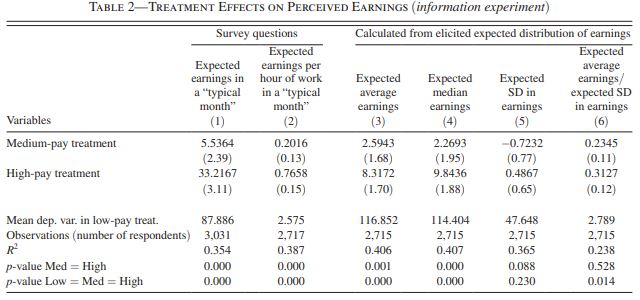
\includegraphics[width=10cm,height=3.25cm]{Deserranno_Table2} 
     \end{figure}
\begin{figure}
     %%%%% this is a minipage, so \textwidth is already adjusted to the size of the column
    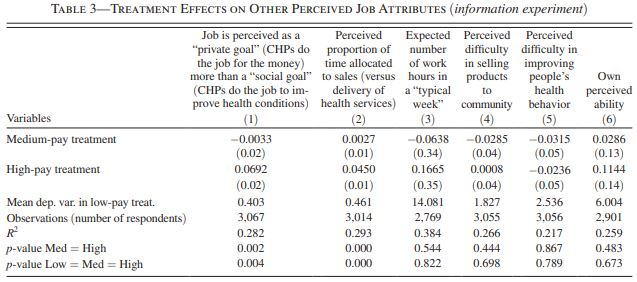
\includegraphics[width=10cm,height=3.25cm]{Deserranno_Table3} 
     \end{figure}



\end{frame}


%------------------------------------------------
\begin{frame}
\frametitle{Recruitment: High Pay Discourages Pro-Social Applicants}
\begin{figure}
     %%%%% this is a minipage, so \textwidth is already adjusted to the size of the column
    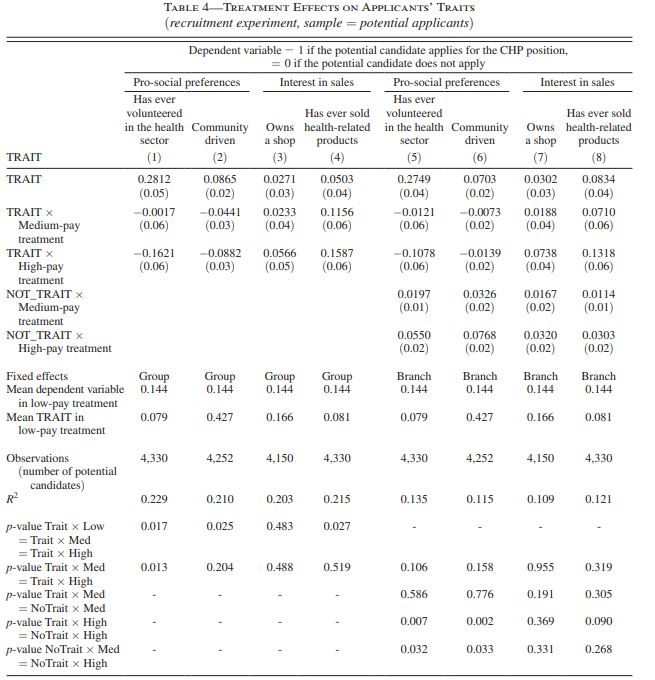
\includegraphics[width=10cm,height=7.5cm]{Deserranno_Table4} 
     \end{figure}






\end{frame}
%adding arbitrary comment
%------------------------------------------------
\begin{frame}
\frametitle{High Pay Treatment Increases Number of Applicants, but Is Associated with Poorer Performance}
\begin{figure}
     %%%%% this is a minipage, so \textwidth is already adjusted to the size of the column
    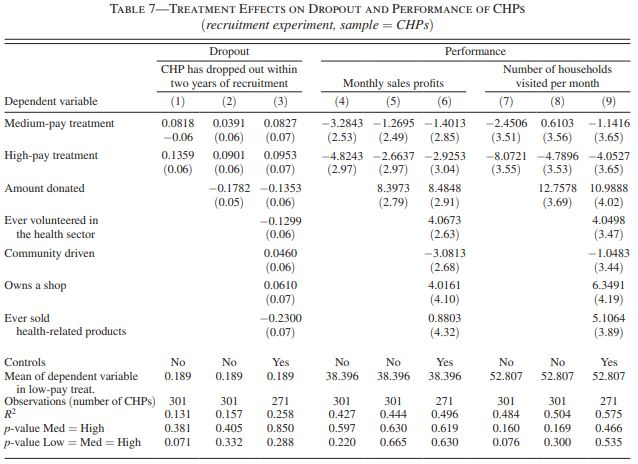
\includegraphics[width=10cm,height=7.5cm]{Deserranno_Table7} 
     \end{figure}



\end{frame}



\end{document} 
